\chapter{Dynamic Memory Management}
\label{chp:dynamic-memory-management}
In order to allow objects to live outside of static scopes, we need to utilize a different memory management technique, such that objects are not allocated on the stack. Dynamic memory management presents a method of storing objects in different memory structures, most commonly, a memory heap. Most irreversible, modern programming languages uses dynamic memory management in some form for allocating space for objects in memory. 

However, reversible, native support for complex data structures is a non-trivial matter to implement. Variable-sized records and frames need to be stored efficiently in a structured heap, while avoiding garbage build-up to maintain reversibility. A reversible heap manager layout has been proposed for a simplified version of the reversible functional language \textsc{RFun} and later expanded to allow references to avoid deep copying values~\cite{ha:heap, ty:rfun, tm:refcounting}.

This chapter presents a brief introduction to fragmentation, garbage and linearity and how these respectively are handled reversibly, and a discussion of various heap manager layouts considered for \rooplpp, along with their advantages and disadvantages in terms of implementation difficulty, garbage build-up and the OOP paradigm. 


\section{Fragmentation}
\label{sec:fragmentation}
Efficient memory usage is an important matter to consider when designing a heap layout for a dynamic memory manager. In a stack allocating memory layout, the stack discipline is in effect, meaning only the most recently allocated data can be freed. This is not the case with heap allocation, where data can be freed regardless of allocation order. A potential side effect of this freedom, comes as a consequence of memory fragmentation. We distinguish different types of fragmentation as internal or external fragmentation. 

Internal fragmentation refers to unused space inside a memory block used to store an object, if, say, the object is smaller than the block it has been allocated to. External fragmentation occurs as blocks freed throughout execution are spread across the memory heap, resulting in \textit{fragmented} free space~\cite{tm:languages}.

\subsection{Internal Fragmentation}
\label{subsec:internal-fragmentation}
Internal fragmentation occurs in the memory heap when part of an allocated memory block is unused. This type of fragmentation can arise from a number of different scenarios, but mostly it originates from cases of \textit{over-allocation}, which occurs when the memory manager delegates memory larger than required to fit an object, due to e.g. fixed-block sizing. 

For an example, consider a scenario, in which we allocate memory for an object of size $m$ onto a simple, fixed-sized block heap. The fixed block size is $n$ and $m \neq n$. If $n > m$, internal fragmentation would occur of size $n-m$ for every object of size $m$ allocated in said heap. If $n < m$, numerous blocks would be required for allocation to fit our object. In this case the internal fragmentation would be of size $n - m\ mod\ n$ per allocated object of size $m$.

\begin{subfigures}
  \begin{figure}[ht]
    \centering
    \begin{tikzpicture}
      % Background
      \fill[fill = grey] (0, 0) rectangle (2, 1) node[midway] {};
  
      % Frame
      \draw (0,0) rectangle (3,1);
      \draw (3,0) rectangle (6,1);
      \draw[dashed] (2, 0) -- (2, 1); 
      
      \draw (1, 0.5) node{Object};
      \draw (4.5, 0.5) node{Free space};
  
      %braces
      \draw[decoration={brace,mirror,raise=5pt},decorate] (0,0) -- node[below=6pt] {$n$} (3,0);
      \draw[decoration={brace,raise=5pt},decorate] (0,1) -- node[above=6pt] {$m$} (2,1);
      \draw[decoration={brace,raise=5pt},decorate] (2,1) -- node[above=6pt] {$n-m$} (3,1); 
    \end{tikzpicture}
    \caption{Creation of internal fragmentation of size $n-m$ due to \textit{over-allocation}}
    \label{fig:internal-frag-example}
  \end{figure}

  \begin{figure}[ht]
    \centering
    \begin{tikzpicture}
      % Background
      \fill[fill = grey] (0, 0) rectangle (4, 1) node[midway] {};
  
      % Frame
      \draw (0,0) rectangle (6,1);
      \draw (6,0) rectangle (9,1);
      \draw[dashed] (4, 0) -- (4, 1);
      
      \draw (2.1, 0.5) node{Object};
      \draw (7.5, 0.5) node{Free space};
  
      %braces
      \draw[decoration={brace,mirror,raise=5pt},decorate] (0,0) -- node[below=6pt] {$n$} (3,0);
      \draw[decoration={brace,raise=5pt},decorate] (0,1) -- node[above=6pt] {$m$} (4,1);
      \draw[decoration={brace,mirror,raise=5pt},decorate] (4,0) -- node[below=6pt] {$n-m\ mod\ n$} (6,0); 
    \end{tikzpicture}
    \caption{Creation of internal fragmentation of size $n-m\ mod\ n$ due to \textit{over-allocation}}
    \label{fig:internal-frag-example-cont}
  \end{figure}
\end{subfigures}

Figure~\ref{fig:internal-frag-example} and~\ref{fig:internal-frag-example-cont} visualize the examples of internal fragmentation build-up from \textit{over-allocating} memory. 

It is difficult for the memory manager to reclaim wasted memory caused by internal fragmentation, as it usually originates from a design choice.
Intuitively, internal fragmentation can best be prevented by ensuring that the size of block(s) being used for allocating space for an object of size $m$ either match or sums to this exact size, when designing the layout. 

\subsection{External Fragmentation}
\label{subsec:external-fragmentation}
External fragmentation materializes in the memory heap when a freed block becomes partly or completely unusable for future allocation if, say, it is surrounded by allocated blocks but the size of the freed block is too small to contain objects on its own.

This type of fragmentation is generally a more substantial cause of problems than internal fragmentation, as the amount of wasted memory typically is larger and less predictable in external fragmentation blocks than in internal fragmentation blocks. Depending on the heap implementation, i.e. a layout using variable-sized blocks of, say, size $2^n$, the internal fragment size becomes considerable for large values of $n$. 

Non-allocatable external fragments become a problem when it is impossible to allocate space for a large object as a result of too many non-consecutive blocks scattered around the heap, caused by the external fragmentation. Physically, there is enough space to store the object, but not in the current heap state. In this scenario we would need to relocate blocks in such a manner that the fragmentation disperses, which is not possible to do reversibly.

Allocation and deallocation order is important in order to combat external fragmentation. For example, if we have a class $A$, which fit on one memory block of size $n$, and we have a class $B$, which fit on two memory blocks of size $n$ and limited memory space, we can easily reach a situation, where we cannot fit more $B$ objects due to external fragmentation.

\begin{figure}[ht]
  \centering
  \begin{subfigure}{.4\textwidth}
    \centering
    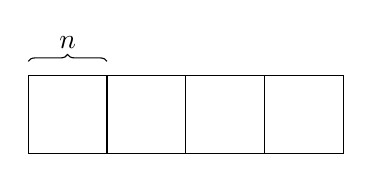
\begin{tikzpicture}
      % Frame
      \draw (0, 0) rectangle (1, 1);
      \draw (1, 0) rectangle (2, 1);
      \draw (2, 0) rectangle (3, 1);
      \draw (3, 0) rectangle (4, 1);

      % Brace
      \draw[decoration={brace,raise=5pt},decorate] (0,1) -- node[above=6pt] {$n$} (1,1);
    \end{tikzpicture}
    \caption{\footnotesize Free memory of size $4n$}
  \end{subfigure}
  \begin{subfigure}{.4\textwidth}
    \centering
    \begin{tikzpicture}
      % Background
      \fill[fill = grey] (0, 0) rectangle (3, 1) node[midway] {};
  
      % Frame
      \draw (0, 0) rectangle (1, 1) node[pos=.5] {$A$};
      \draw (1, 0) rectangle (3, 1) node[pos=.5] {$B$};
      \draw (3, 0) rectangle (4, 1);

      % Braces
      \draw[decoration={brace,raise=5pt},decorate] (0,1) -- node[above=6pt] {$n$} (1,1);
      \draw[decoration={brace,raise=5pt},decorate] (1,1) -- node[above=6pt] {$2n$} (3,1);
    \end{tikzpicture}
    \caption{\footnotesize Allocate $A$ and $B$}
  \end{subfigure}
  \vskip 1em
  \begin{subfigure}{.6\textwidth}
    \centering
    \begin{tikzpicture}
      % Background
      \fill[fill = grey] (1, 0) rectangle (3, 1) node[midway] {};
  
      % Frame
      \draw (0, 0) rectangle (1, 1);
      \draw (1, 0) rectangle (3, 1) node[pos=.5] {$B$};
      \draw (3, 0) rectangle (4, 1);
    \end{tikzpicture}
    \caption{\footnotesize Free $A$. Cannot fit another $B$ due to external fragmentation}
  \end{subfigure}
  \caption{Example of external fragmentation caused for allocation and deallocation order}
  \label{fig:external-frag-example}
\end{figure}  

Figure~\ref{fig:external-frag-example} shows this example, where the allocation and deallocation order causes a situation, in which we cannot allocate any more $B$ objects, even though we physically have the required amount of free space in memory. 

\begin{figure}[ht]
  \centering
  \begin{subfigure}{.4\textwidth}
    \centering
    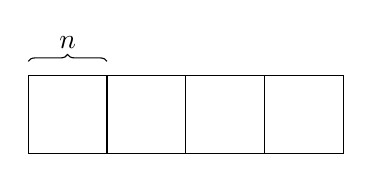
\begin{tikzpicture}
      % Frame
      \draw (0, 0) rectangle (1, 1);
      \draw (1, 0) rectangle (2, 1);
      \draw (2, 0) rectangle (3, 1);
      \draw (3, 0) rectangle (4, 1);

      % Brace
      \draw[decoration={brace,raise=5pt},decorate] (0,1) -- node[above=6pt] {$n$} (1,1);
    \end{tikzpicture}
    \caption{\footnotesize Free memory of size $4n$}
  \end{subfigure}
  \begin{subfigure}{.4\textwidth}
    \centering
    \begin{tikzpicture}
      % Background
      \fill[fill = grey] (0, 0) rectangle (3, 1) node[midway] {};
  
      % Frame
      \draw (0, 0) rectangle (2, 1) node[pos=.5] {$B$};
      \draw (2, 0) rectangle (3, 1) node[pos=.5] {$A$};
      \draw (3, 0) rectangle (4, 1);

      % Braces
      \draw[decoration={brace,raise=5pt},decorate] (0,1) -- node[above=6pt] {$2n$} (2,1);
      \draw[decoration={brace,raise=5pt},decorate] (2,1) -- node[above=6pt] {$n$} (3,1);
    \end{tikzpicture}
    \caption{\footnotesize Allocate $B$ and $A$}
  \end{subfigure}
  \vskip 1em
  \begin{subfigure}{.4\textwidth}
    \centering
    \begin{tikzpicture}
      % Background
      \fill[fill = grey] (0, 0) rectangle (2, 1) node[midway] {};
  
      % Frame
      \draw (0, 0) rectangle (2, 1) node[pos=.5] {$B$};
      \draw (2, 0) rectangle (3, 1);
      \draw (3, 0) rectangle (4, 1);
    \end{tikzpicture}
    \caption{\footnotesize Free $A$}
  \end{subfigure}
  \begin{subfigure}{.4\textwidth}
    \centering
    \begin{tikzpicture}
      % Background
      \fill[fill = grey] (0, 0) rectangle (4, 1) node[midway] {};
  
      % Frame
      \draw (0, 0) rectangle (2, 1) node[pos=.5] {$B$};
      \draw (2, 0) rectangle (4, 1) node[pos=.5] {$B$};
    \end{tikzpicture}
    \caption{\footnotesize Allocate another $B$}
  \end{subfigure}
  \caption{Example of avoiding external fragmentation using allocation and deallocation order}
  \label{fig:external-frag-example-cont}
\end{figure}  

Figure~\ref{fig:external-frag-example-cont} shows how changing allocation and deallocation order can combat external fragmentation.

\section{Memory Garbage}
\label{sec:memory-garbage}
A reversible computation should be garbage-free and as such it should be our goal to return the memory to its original state after program termination.

Traditionally, in non-reversible programming languages, freed memory blocks are simply re-added to the free list during deallocation and no modification of the actual data stored in the block is performed, as it simply is overwritten when the block is used later on. In the reversible setting we must return the memory block to its original state after the block has been freed (e.g. zero-cleared), to uphold the time-invertible and two-directional computational model. Figure~\ref{fig:injective-garbage-in-out} illustrates how the output data (or garbage) of an injective function $f$ is the input to its inverse function $f^{-1}$.

In heap allocation layouts, we maintain one or more free lists to keep track of free blocks during program execution, which are stored in memory, besides the heap representation itself. These free lists can essentially be considered garbage and as such, they must also be returned to their original state after execution. Furthermore, the heap itself can also be considered garbage and if it grows during execution, it should also be returned to its original size.

\begin{figure}[ht]
  \centering
    \begin{tikzpicture}
      % lines
      \draw[-] (-1,1.75) node[left]{$in$} -- (9,1.75) node[right] {$in$};
      \draw[-] (2,1.25) -- (6,1.25);
      \draw[-] (2,0.75) -- (6,0.75);
      \draw[-] (2,0.25) -- (6,0.25);
      \draw[-] (-1,-0.5) node[left]{$out$} -- (9,-0.5) node[right] {$out$};
      \draw[-] (4,0.24) node[circle,fill,inner sep=1pt] {} -- (4,-0.5) node[circle,fill,inner sep=1pt] {};
      
      % boxes
      \draw[fill = white] (0, 0) rectangle (2, 2) node[pos=0.5] {\Large $f$};
      \draw[fill = white] (6, 0) rectangle (8, 2) node[pos=0.5] {\Large $f^{-1}$};
      \node[diamond, fill=white, draw] at (4,1.25) {\scriptsize $garbage$};
    \end{tikzpicture}
    \caption{The "garbage" output of an injective function $f$ is the input to its inverse function $f^{-1}$}
    \label{fig:injective-garbage-in-out}
\end{figure}

Returning the free list(s) to their original states is a non-trivial matter, which is highly dependent on the heap layout and free list design.~\citeauthor{ha:heap} introduced a dynamic memory manager which allowed heap allocation and deallocation, but without restoring the free list to its original state in~\cite{ha:heap}.~\citeauthor{ha:heap} argue that an unrestored free list can be considered harmless garbage in the sense that the free list residing in memory after termination is equivalent to a restored free list, as it contains the same blocks, but linked in a different order, depending on the order of allocation and deallocation operations performed during program execution. Figure~\ref{fig:equivalent-free-lists} illustrates how an inverse, injective function $f^{-1}$, whose non-inverse function $f$ computes something which modifies a given free lists, does not require the \textit{exact} output free list of $f$, but \textit{any} free list of same layout as input for the inverse function $f^{-1}$. The output free list of $f^{-1}$ will naturally be a further modified free list.

\begin{figure}[ht]
  \centering
  % 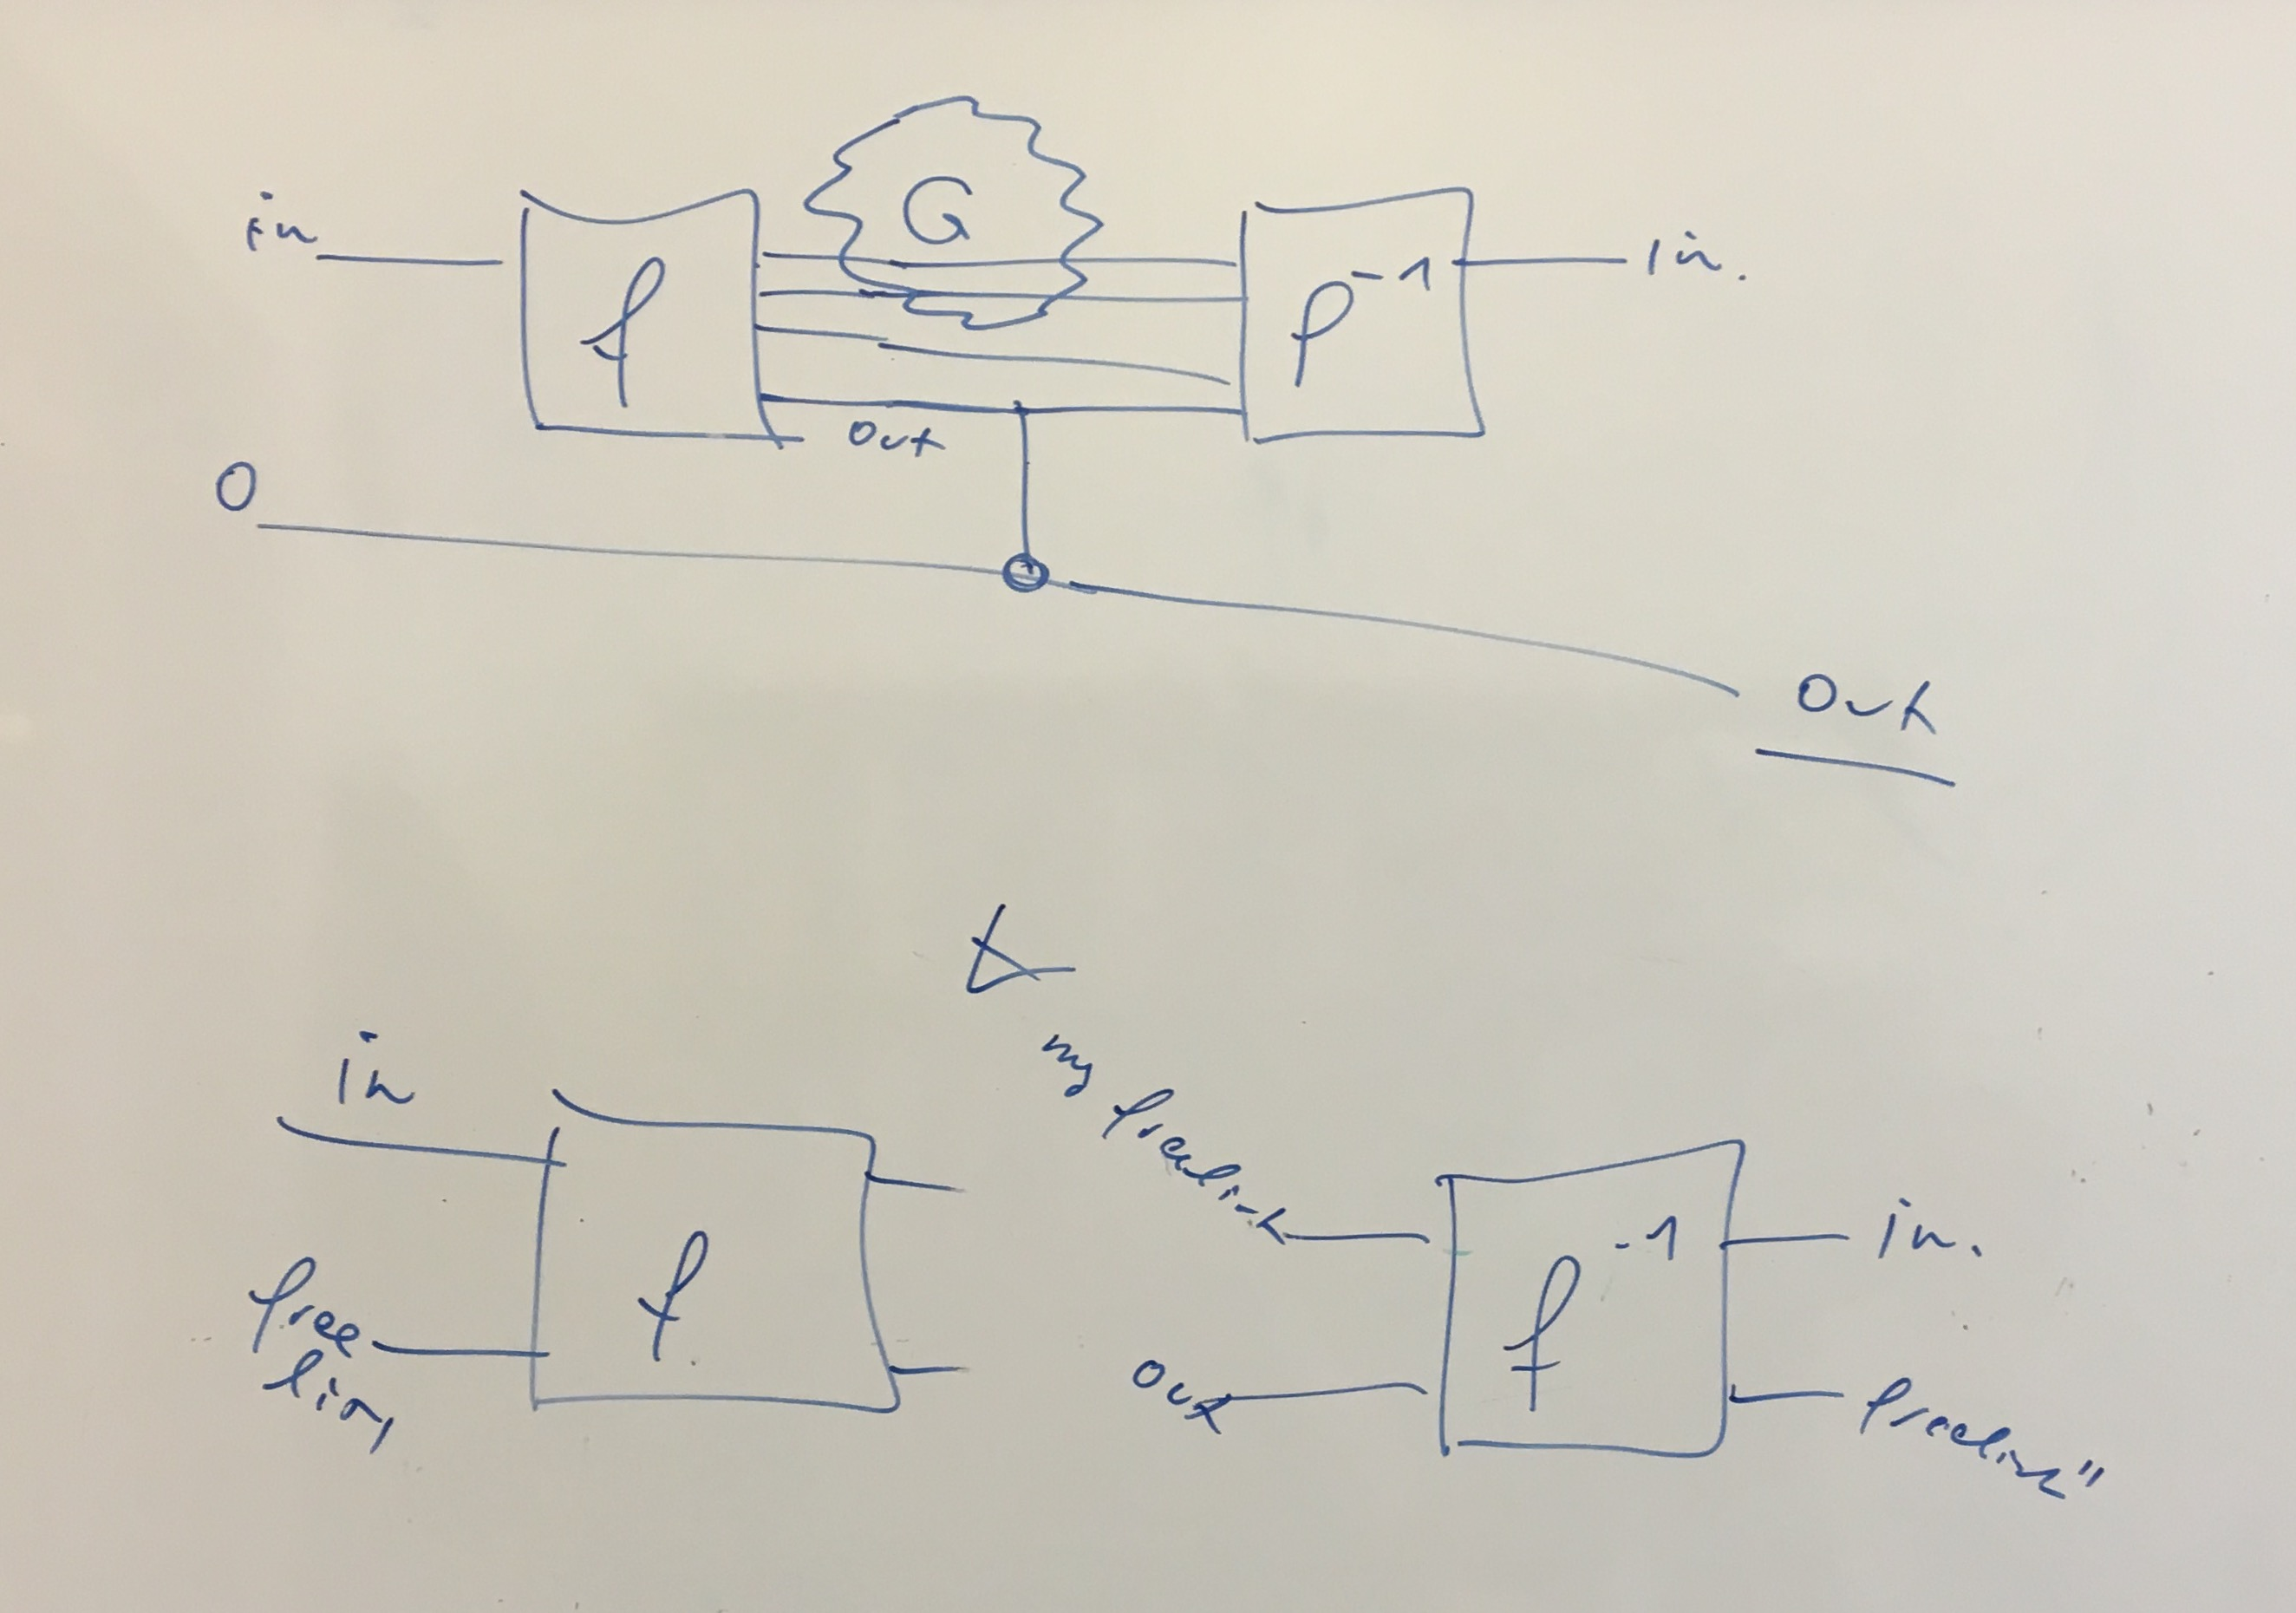
\includegraphics[width=0.7\textwidth]{garbage-classes}
  \begin{tikzpicture}
    % lines
    \draw[-] (-1,1.75) node[left]{$free\ list$} -- (2,1.75);
    \draw[-] (-1,0.25) node[left]{$in$} -- node[below] {$out$} (10,0.25) node[right] {$in$};
    \draw (7,1.75) .. controls (6,1.75) and (6,1.75) .. (6,2.75) node[above] {$\forall\ free\ lists$};
    \draw (2,1.75) .. controls (3,1.75) and (3,1.75) .. (3,2.75) node[above] {$free\ list'$};
    \draw[-] (9,1.75) -- (10,1.75) node[right]{$free\ list''$};
    
    % boxes
    \draw[fill = white] (0, 0) rectangle (2, 2) node[pos=0.5] {\Large $f$};
    \draw[fill = white] (7, 0) rectangle (9, 2) node[pos=0.5] {\Large $f^{-1}$};
  \end{tikzpicture}
  \caption{All free lists are considered equivalent "garbage" in terms of injective functions}
  \label{fig:equivalent-free-lists}
\end{figure}

This intuitively leads to the question of garbage classification. In the reversible setting all functions are injective. Thus, given some $input_f$, in a reversible computation using heap allocation, the injective function $f$ produces some $output_f$ and some $garbage_f$ (e.g. garbage in form of storing data in the heap, so the free list changes, the heap grows, etc.). Its inverse function $f^{-1}$ must thus take the $output_f$ of $f$ and $garbage_f$ as $input_{f^{-1}}$ to produce its output $output_{f^{-1}}$ which is the $input_f$ of $f$. However, in the context of reversible heaps, we must consider all free lists as of "equivalent garbage class" and thus freely substitutable with each other, as injective functions still can drastically change the block layout, free list order, etc. during its execution in either direction. Figure~\ref{fig:equivalent-free-lists} shows how any free list can be passed between a function $f$ and its inverse $f^{-1}$.


\section{Linearity and Reference Counting}
\label{sec:referencing}
Programming languages use different approaches for storing and synchronizing variables and objects in memory. Typing \textit{linearity} is a distinction, which can reduce storage management and synchronization costs~\cite{hb:linearity}.

Reversible programming languages such as \textsc{Janus} and \textsc{Roopl} are linear in the sense that object and variable pointers cannot be copied and are only deleted during deallocation. Pointer copying greatly increases the flexibility of programming, especially in a reversible settings where zero-clearing is critical, at the cost of increased management in form of reference counting for e.g. objects. For variables, pointer copying is not particular interesting, nor would it add much flexibility as the values of a variable simply can be copied into statically-scoped local blocks. For objects however, tedious amounts of boilerplate work must be done if object $A$ and $B$ need to work on the same object $C$ and only one reference to each object is allowed.

\citeauthor{tm:refcounting} presented the reversible functional language \textsc{Rcfun} which use reference counting to allow multiple pointers to the same memory nodes as well as a translation from \textsc{Rcfun} into \textsc{Janus} in \cite{tm:refcounting}. In \textsc{Rcfun}, reference counting is used to manage and trace the number of pointer copies made by respectively incrementing and decrementing a \textit{reference count} stored in the memory node, whenever the original node pointer is copied or a copy pointer is deleted. For the presented heap manage, deletion of object nodes was only allowed when no references to a node remained.

In non-reversible languages, reference counting is also used in garbage collection by automatically deallocating unreachable objects and variables which contains no referencing. 


\section{Heap Manager Layouts}
\label{sec:heap-manager-layout}
Heap managers can be implemented in numerous ways. Different layouts yield advantages when allocating memory, finding a free block or when collecting garbage. As our goal is to construct a garbage-free heap manager, our finalized design should emphasize and reflect this objective in particular. Furthermore, we should attempt to allocate and deallocate memory as efficiently as possible, as merging and splitting of blocks is a non-trivial problem in a reversible setting and to avoid problematic fragmentation.

For the sake of simplicity, we will not consider the issue of retrieving memory pages reversibly. A reversible operating system is a long-term dream of the reversible researcher and as reversible programming language designers, we assume that \rooplpp will be running in an environment, in which an operating system will be supplying memory pages and their mappings. As such, the following heap memory designs reflect this preliminary assumption, that we can always query the operating system for more memory. 

Historically, most object-oriented programming languages utilize a dynamic memory manager during program execution. In older, lower-level languages such as \textsc{C}, memory management is manual and allocation has to be stated explicitly and with the requested size through the \textbf{malloc} statement and deallocated using the \textbf{free} statement. Modern languages, such as \textsc{C\texttt{++}}, \textsc{Java} and \textsc{Python}, \textit{automagically} allocates and frees space for objects and variable-sized arrays by utilizing their dynamic memory manager and garbage collector to dispatch \textbf{malloc}- and \textbf{free}-like operations to the operating system and managing the obtained memory blocks in private heap(s)~\cite{wh:cpp_memory, bv:jvm, py:memory}. The heap layout of these managers vary from language to language and compiler to compiler.

Previous work on reversible heap manipulation has been done for reversible functional languages in~\cite{ha:heap, jsk:translation, tm:garbage}.

\citeauthor{ha:heap} presented a static heap structure consisting of \textsc{Lisp}-inspired constructor cells of fixed size and a single free list for the reversible function language \textsc{Rfun} in~\cite{ha:heap}. \citeauthor{tm:refcounting} presented an implementation in \textsc{Janus} of reversible reference counting under the assumption of \citeauthor{ha:heap}'s heap manager in~\cite{tm:refcounting}. Building on the previous work, \citeauthor{tm:garbage} later presented a reversible intermediate language \textsc{Ril} and an implementation in \textsc{Ril} of a reversible heap manager, which uses reference counting and hash-consing to achieve garbage collection in~\cite{tm:garbage}.

We do not consider reference counting or garbage collection in the layouts presented in the following sections, but we later show how the selected layout for \rooplpp is extended with reference counting in section~\ref{sec:referencing-compilation}.

\subsection{Memory Pools}
\label{subsec:memory-pools}
The simplest heap layout we can design uses fixed-sized blocks. This design is also known as memory pools, as memory is allocated from "pools" of fixed-sized blocks regardless of the record size.
To model these pools of fixed-sized blocks, we simply use a linked list of identically sized free block cells, which we maintain over execution.
While the fixed-block layout is simple and relatively easy in terms of implementation it is also largely uninteresting as it provides little to no options, besides sizing of the fixed-blocks, to combat fragmentation.

This layout comes with a few options in terms of the actual heap layout. If we only allow allocation of consecutive, adjacent free blocks, we should keep the free list sorted. If the free list is not sorted, and we have to allocate an object which requires $n$ blocks, we have to iterate the free list $n^2$ times in the worst case to find a chain of consecutive blocks large enough to fit the object. The sorting part itself is non-trivial matter. Furthermore, we need some overhead storage inside the object to contains the references of the blocks occupied by the object, or some other structure which can be used when deallocating the object and returning all the blocks to the free list. If we allow allocation of non-consecutive blocks, larger amounts of bookkeeping is required as we need to store knowledge of when and where the object is split.

Figures~\ref{fig:external-frag-example} and~\ref{fig:external-frag-example-cont} from earlier in this chapter, in section~\ref{subsec:external-fragmentation} on page~\pageref{fig:external-frag-example} illustrates examples with consecutive, fixed-sized block allocation. 


\subsection{One Heap Per Record Size}
\label{subsec:one-heap-per-record-size}
Instead of allocating space for objects from a single free list and heap, we could design an approach which uses one heap per record size, known as a multi-heap layout. The respective classes and their sizes are easily identified during compile time from which the amount of heaps and free list will be initialized. This means the layout is very dynamic and potentially can change drastically in terms of the amount of heaps utilized depending on the input program. 

\begin{figure}[ht]
  \centering
  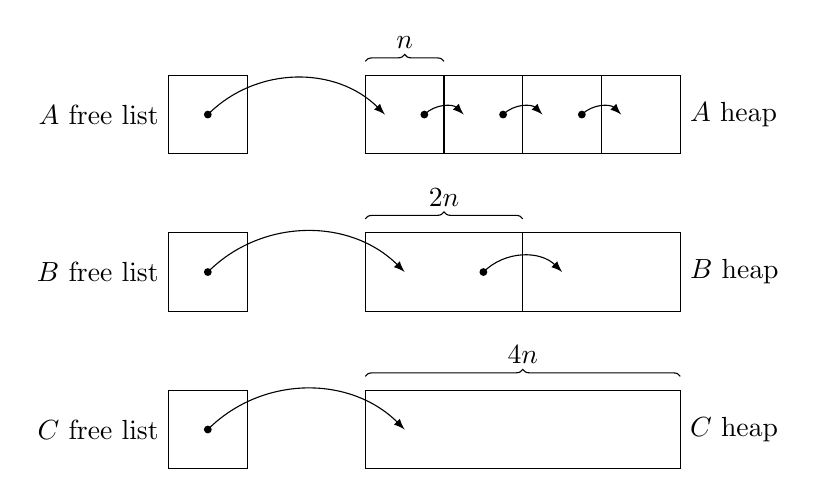
\begin{tikzpicture}
    % Heaps
    \draw[step=1cm] (0,4) grid (4,5);
    \node[right] at (4,4.5) {$A$ heap}; 
    \draw (0,2) rectangle (2,3) rectangle node[right, xshift=1cm] {$B$ heap} (4,2);
    \draw (0,0) rectangle node[right, xshift=2cm] {$C$ heap} (4,1);

    % Free lists
    \draw (-2.5, 4) rectangle node[left, xshift=-0.5cm] {$A$ free list} (-1.5, 5);
    \draw (-2.5, 2) rectangle node[left, xshift=-0.5cm] {$B$ free list} (-1.5, 3);
    \draw (-2.5, 0) rectangle node[left, xshift=-0.5cm] {$C$ free list} (-1.5, 1);
    
    % Arrow for 1st heap pair
    \node[circle,fill,inner sep=1pt] at (-2, 4.5) {};
    \draw[-latex] (-2, 4.5) to[out=45, in=135] (0.25, 4.5);
    \node[circle,fill,inner sep=1pt] at (0.75, 4.5) {};
    \draw[-latex] (0.75, 4.5) to[out=45, in=135] (1.25, 4.5);
    \node[circle,fill,inner sep=1pt] at (1.75, 4.5) {};
    \draw[-latex] (1.75, 4.5) to[out=45, in=135] (2.25, 4.5);
    \node[circle,fill,inner sep=1pt] at (2.75, 4.5) {};
    \draw[-latex] (2.75, 4.5) to[out=45, in=135] (3.25, 4.5);

    % Arrow for 2nd heap pair
    \node[circle,fill,inner sep=1pt] at (-2, 2.5) {};
    \draw[-latex] (-2, 2.5) to[out=45, in=135] (0.5, 2.5);
    \node[circle,fill,inner sep=1pt] at (1.5, 2.5) {};
    \draw[-latex] (1.5, 2.5) to[out=45, in=135] (2.5, 2.5);

    % Arrow for 3rd heap pair
    \node[circle,fill,inner sep=1pt] at (-2, 0.5) {};
    \draw[-latex] (-2, 0.5) to[out=45, in=135] (0.5, 0.5);

    % Braces
    \draw[decoration={brace,raise=5pt},decorate] (0,1) -- node[above=6pt] {$4n$} (4,1);
    \draw[decoration={brace,raise=5pt},decorate] (0,3) -- node[above=6pt] {$2n$} (2,3);
    \draw[decoration={brace,raise=5pt},decorate] (0,5) -- node[above=6pt] {$n$} (1,5);
  \end{tikzpicture}
  \caption{Memory layout using one heap per record size}
  \label{fig:one-heap-per-record-size}
\end{figure}

Figure~\ref{fig:one-heap-per-record-size} illustrates three heaps with respective free lists for three classes $A$, $B$ and $C$ of size $n$, $2n$ and $4n$. Each heap is represented as a simple linked list with the free list simply being a pointer to the first free block in the heap. 

The advantage of this approach would be effective elimination of internal and external fragmentation, as each heap fits their targeted record perfectly, making each allocation and deallocation tailored to the size of the record obtained from a static analysis during compilation, resulting in no over-allocation and no unusable chunks of freed memory appearing during varying deallocation order. Implementation-wise, allocation of an object of a given class simply becomes the task of popping the head of the respective free list, which can easily be determined at compile time. The deallocation is simply adding a new head to the free list.

Listing~\ref{lst:one-heap-per-record-size} outlines the allocation algorithm for this layout written in extended \textsc{Janus} from~\cite{ty:ejanus}. We assume that the heads of the free lists are stored in a single array primitive, such that the free list for records of size $n$ are indexed at $n-2$ and $n > 2$ (as every record needs some overhead) and that we have heaps for continuous size range with no gaps. To maintain reversibility we only allow allocation from the head of the free list.

The algorithm consists of an entry point named \textbf{malloc} and a recursion body named \textbf{malloc1}. Given a zero-cleared pointer $p$, the size of the object we are allocating $o_{size}$ and the array of free lists primitive, the recursion body is called after initializing a $counter$, which is an index into the free lists array and a counter size, $c_{size}$, which is the block size of the current free list the $counter$ is indexed in. The recursion body first updates the free list index until we find a free list with a size greater or equal to the size of the object we are allocating. Once such a free list has been found, the head of the free list is simply popped and the next block is set as the new head.\\

\begin{lstlisting}[caption={Allocation algorithm for one heap per record size implemented in extended Janus}, language=janus, style=basic, label={lst:one-heap-per-record-size}]
  procedure malloc(int p, int osize, int freelists[])
    local int counter = 0
    local int csize = 2
    call malloc1(p, osize, freelists, counter, csize)
    delocal int csize = 2
    delocal int counter = 0

  procedure malloc1(int p, int osize, int freelists[], int counter, int csize)
    if (csize < osize) then
      counter += 1
      csize += 1
      call malloc1(p, osize, freelists, counter, csize) 
      csize -= 1
      counter -= 1
    else
      p += freelists[counter]
      freelists[counter] -= p

      // Swap head of free list with next block of p 
      freelists[counter] ^= M(p)
      M(p) ^= freelists[counter]
      freelists[counter] ^= M(p)
    fi csize < osize   
\end{lstlisting}

The obvious disadvantage to this layout is the amount of bookkeeping and workload associated with growing and shrinking a heap and its neighbours, in case the program requests additional memory from the operating system. In real world object-oriented programming, most classes feature a small number of fields, very rarely more than 16. 

Additionally, helper classes of other sizes would spawn additional heaps and bookkeeping work, making the encapsulation concept of OOP rather unattractive, for the optimization-oriented reversible programmer. 

Finally, while internal and external fragmentation is effectively eliminated, we are left with additional and considerable amounts of garbage in forms of all the heaps and free lists initialized in memory. If two record types only differ one word in size, two heaps would be initialized. Each heap intuitively need to be initialized with a chunk of memory from the underlying operating system such that objects can be allocated on their respective heaps, regardless of the number of times the heap is used during program execution. This is an obvious space requirement increase over the previously presented layout, and on average, the amount of required memory for a program compiled using this approach would probably be larger, than some of the following layouts, due to unoptimized heap utilization and sharing.


\subsection{One Heap Per Power-Of-Two}
\label{subsec:one-heap-per-power-of-two}
To address the issues of the previous heap manager layout, we can optimize the amounts of heaps required by introducing a relatively small amount of internal fragmentation. Instead of having a heap per record size, we could have a heap per power-of-two. Records would be stored in the heap closest to their respective size and as such, we reduce the number of heaps needed, as many different records can be stored in the same heap. Records of size $5$, $6$, $7$ and $8$ would in the former layout be stored in four different heaps, where they would be stored in a single heap using this layout. Figure~\ref{fig:one-heap-per-power-of-two} illustrates the free lists and heaps up to $n^m$. 

\begin{figure}[ht]
  \centering
  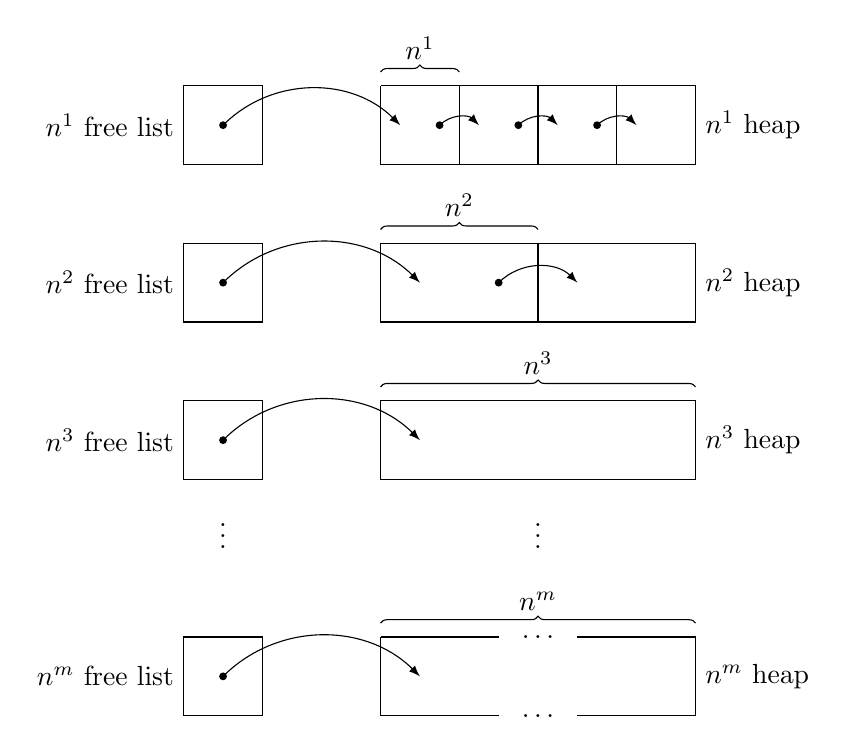
\begin{tikzpicture}
    % Heaps
    \draw[step=1cm] (0,4) grid (4,5);
    \node[right] at (4,4.5) {$n^1$ heap}; 
    \draw (0,2) rectangle (2,3) rectangle node[right, xshift=1cm] {$n^2$ heap} (4,2);
    \draw (0,0) rectangle node[right, xshift=2cm] {$n^3$ heap} (4,1);

    \draw (0,-3) -- (0, -2);
    \draw (0,-3) -- (1.5, -3);
    \draw (0,-2) -- (1.5, -2);
    \draw (2.5,-3) -- (4, -3);
    \draw (2.5,-2) -- (4, -2);
    \draw (4,-3) -- (4, -2);
    \node[right] at (4,-2.5) {$n^m$ heap};  

    % Free lists
    \draw (-2.5, 4) rectangle node[left, xshift=-0.5cm] {$n^1$ free list} (-1.5, 5);
    \draw (-2.5, 2) rectangle node[left, xshift=-0.5cm] {$n^2$ free list} (-1.5, 3);
    \draw (-2.5, 0) rectangle node[left, xshift=-0.5cm] {$n^3$ free list} (-1.5, 1);
    \draw (-2.5, -3) rectangle node[left, xshift=-0.5cm] {$n^m$ free list} (-1.5, -2);
    
    % Arrow for 1st heap pair
    \node[circle,fill,inner sep=1pt] at (-2, 4.5) {};
    \draw[-latex] (-2, 4.5) to[out=45, in=135] (0.25, 4.5);
    \node[circle,fill,inner sep=1pt] at (0.75, 4.5) {};
    \draw[-latex] (0.75, 4.5) to[out=45, in=135] (1.25, 4.5);
    \node[circle,fill,inner sep=1pt] at (1.75, 4.5) {};
    \draw[-latex] (1.75, 4.5) to[out=45, in=135] (2.25, 4.5);
    \node[circle,fill,inner sep=1pt] at (2.75, 4.5) {};
    \draw[-latex] (2.75, 4.5) to[out=45, in=135] (3.25, 4.5);

    % Arrow for 2nd heap pair
    \node[circle,fill,inner sep=1pt] at (-2, 2.5) {};
    \draw[-latex] (-2, 2.5) to[out=45, in=135] (0.5, 2.5);
    \node[circle,fill,inner sep=1pt] at (1.5, 2.5) {};
    \draw[-latex] (1.5, 2.5) to[out=45, in=135] (2.5, 2.5);

    % Arrow for 3rd heap pair
    \node[circle,fill,inner sep=1pt] at (-2, 0.5) {};
    \draw[-latex] (-2, 0.5) to[out=45, in=135] (0.5, 0.5);

    % Arrow for 4th heap pair
    \node[circle,fill,inner sep=1pt] at (-2, -2.5) {};
    \draw[-latex] (-2, -2.5) to[out=45, in=135] (0.5, -2.5);

    % Braces
    \draw[decoration={brace,raise=5pt},decorate] (0,5) -- node[above=6pt] {$n^1$} (1,5);
    \draw[decoration={brace,raise=5pt},decorate] (0,3) -- node[above=6pt] {$n^2$} (2,3);
    \draw[decoration={brace,raise=5pt},decorate] (0,1) -- node[above=6pt] {$n^3$} (4,1);
    \draw[decoration={brace,raise=5pt},decorate] (0,-2) -- node[above=6pt] {$n^m$} (4,-2);

    % Dots
    \node[above] at (-2, -1) {$\vdots$};
    \node[above] at (2, -1) {$\vdots$};
    \node[] at (2, -2) {$\dots$};
    \node[] at (2, -3) {$\dots$};
  \end{tikzpicture}
  \caption{Memory layout using one heap per power-of-two}
  \label{fig:one-heap-per-power-of-two}
\end{figure}

Internal fragmentation does become a problem for very large records, as blocks are only of size $2^n$. An object of size $65$ would fit in a $128$ sized block, resulting in considerable amounts of wasted memory space in form of internal fragmentation. However, in the real world, most records are small and allocation of records causing this much amount of fragmentation is an unlikely scenario. To avoid large amounts of internal fragmentation building up when allocating large records, we could allocate space for large objects using smaller blocks. If a record exceeds some limit, which has been determined the cutoff point, one kilobyte for an example, we could split it into $\sqrt{n}$ sized chunks and use blocks of that size instead. This would reduce the amount of internal fragmentation at the cost of increased bookkeeping.
For smaller records, very minimal amounts of internal fragmentation occur. 

The number of heaps needed for a computation can be determined at compile time by finding the smallest and largest record sizes and ensuring we have heaps to fit these effectively. The allocation process consists of determining the closest $2^n$ to the size of the record we are allocating and then simply popping the head of the respective free list.

Listing~\ref{lst:one-heap-per-power-of-two} shows a modified \textbf{malloc1} recursion body for the power-of-two approach. Once again, we assume our array of free lists contains the head of each free list, such that index $n$ is the head of the free list of size $2^{n+1}$. Instead of incrementing the counter size by one, as in the former layout algorithm, we double it, using the shown \textbf{double} procedure. Besides this change, the algorithm remains unchanged and still assumes each heap has been initialized along with the free lists.\\

\begin{lstlisting}[caption={Allocation algorithm for one heap per power-of-two implemented in extended Janus}, language=janus, style=basic, label={lst:one-heap-per-power-of-two}]
  procedure double(int target)
    local int current = target
    target += current
    delocal int current = target / 2

  procedure malloc1(int p, int osize, int freelists[], int counter, int csize)
    if (csize < osize) then
        counter += 1
        call double(csize)
        call malloc1(p, osize, freelists, counter, csize) 
        uncall double(csize)
        counter -= 1
    else
      if freelists[counter] != 0 then
        p += freelists[counter]
        freelists[counter] -= p

        // Swap head of free list with next block of p
        freelists[counter] ^= M(p)
        M(p) ^= freelists[counter]
        freelists[counter] ^= M(p)
      else
        counter += 1
        call double(csize)
        call malloc1(p, osize, freelists, counter, csize)
        uncall double(csize)
        counter -= 1
      fi freelists[counter] = 0 || p != freelists[counter]
    fi csize < osize   
\end{lstlisting}


\subsection{Shared Heap, Record Size-Specific Free Lists}
\label{subsec:shared-heap}
A natural proposal, considering the disadvantages of the previously presented designs, would be using a shared heap instead of record-specific heaps. 
This way, we ensure minimal fragmentation when allocating and freeing as the different free lists ensure that allocation of an object wastes as little memory as possible. By only keeping one heap, we eliminate the growth/shrinking issues of the multiple heap layout. 

There is, however, still a considerable amount of bookkeeping involved in maintaining multiple free lists. Having mixed-size blocks in a single heap is also a task which might prove difficult to accomplish reversibly. How initialization and destruction of said heap should work is not clear. As with the multiple heap version of this layout, we are still left with the issues surrounding two records which only differs one word in size. In the former layout, two heaps were required to store records of these types. In this layout, we need to store two block sizes in our heap to allocate these records, with no internal fragmentation. We could allow these objects to be allocated on similarly-sized blocks, if we round the calculated class sizes up to, say, a power-of-two. We would essentially have a shared heap, power-of-two-specific free lists layout.

\begin{figure}[ht]
  \centering
  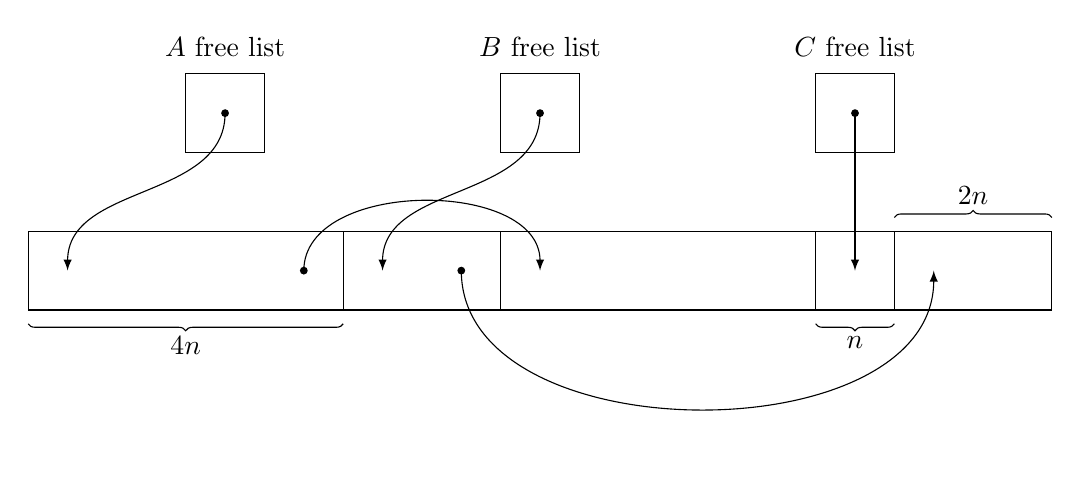
\begin{tikzpicture}
    % Heap
    \draw (0, 0) rectangle (4, 1);
    \draw (4, 0) rectangle (6, 1);
    \draw (6, 0) rectangle (10, 1);
    \draw (10, 0) rectangle (11, 1);
    \draw (11, 0) rectangle (13, 1);

    % Free lists
    \draw (2, 2) rectangle (3, 3) node[midway, above, yshift=0.6cm] {$A$ free list}; 
    \draw (6, 2) rectangle (7, 3) node[midway, above, yshift=0.6cm] {$B$ free list};
    \draw (10, 2) rectangle (11, 3) node[midway, above, yshift=0.6cm] {$C$ free list};

    % Arrows 1st heap
    \node[circle,fill,inner sep=1pt] at (2.5, 2.5) {};
    \draw[-latex] (2.5, 2.5) to[out=270, in=90] (0.5, 0.5);

    \node[circle,fill,inner sep=1pt] at (3.5, 0.5) {};
    \draw[-latex] (3.5, 0.5) to[out=90, in=90] (6.5, 0.5);

    % Arrows 2nd heap
    \node[circle,fill,inner sep=1pt] at (6.5, 2.5) {};
    \draw[-latex] (6.5, 2.5) to[out=270, in=90] (4.5, 0.5);

    \node[circle,fill,inner sep=1pt] at (5.5, 0.5) {};
    \draw[-latex] (5.5, 0.5) to[out=-90, in=-90] (11.5, 0.5);

    % Arrows 3rd heap
    \node[circle,fill,inner sep=1pt] at (10.5, 2.5) {};
    \draw[-latex] (10.5, 2.5) to[out=270, in=90] (10.5, 0.5);

    % Braces
    \draw[decoration={brace, mirror, raise=5pt},decorate] (0,0) -- node[below=6pt] {$4n$} (4,0);
    \draw[decoration={brace, mirror, raise=5pt},decorate] (10,0) -- node[below=6pt] {$n$} (11,0);
    \draw[decoration={brace, raise=5pt},decorate] (11,1) -- node[above=6pt] {$2n$} (13,1);
  \end{tikzpicture}
  \caption{Record size-specific free lists on a shared heap}
  \label{fig:shared-heap}
\end{figure}

As the only change in this design are the heaps themselves, the allocation process remains unchanged from the one presented in listing~\ref{lst:one-heap-per-record-size} or listing~\ref{lst:one-heap-per-power-of-two} if we use the power-of-two approach. Figure~\ref{fig:shared-heap} visualizes the shared heap and the free lists of this layout.


\subsection{Buddy Memory}
\label{subsec:buddy-memory}
The Buddy Memory layout utilizes blocks of variable-sizes of the power-of-two, typically with one free list per power-of-two using a shared heap. When allocating an object of size $m$, we simply check the free lists for a free block of size $n$, where $n \geq m$. Is such a block found and if $n > m$, we split the block into two halves recursively, until we obtain the smallest block capable of storing $m$. When deallocating a block of size $m$, we do the action described above in reverse, thus merging the blocks again, where possible.

\begin{figure}[ht]
  \centering
  \begin{subfigure}{.5\textwidth}
    \centering
    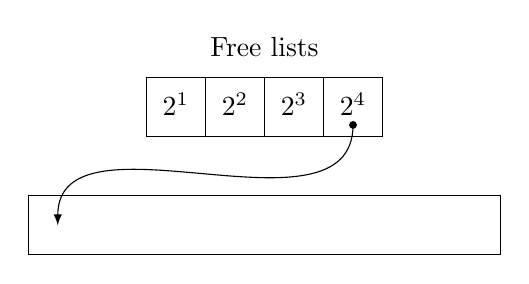
\begin{tikzpicture}[scale=0.75]
      % Boxes
      \draw[step=1] (2,2) grid (6,3);
      \draw (0,0) rectangle (8, 1);

      % Labels
      \node[above] at (4, 3.2) {Free lists}; 
      \node[above] at (2.5, 2.2) {$2^1$}; 
      \node[above] at (3.5, 2.2) {$2^2$}; 
      \node[above] at (4.5, 2.2) {$2^3$}; 
      \node[above] at (5.5, 2.2) {$2^4$}; 
      
      % Arrows
      \node[circle,fill,inner sep=1pt] at (5.5, 2.2) {};
      \draw[-latex] (5.5, 2.2) to[out=270, in=90] (0.5, 0.5);
    \end{tikzpicture}
    \caption{\footnotesize Initial memory block}
  \end{subfigure}%
  \begin{subfigure}{.5\textwidth}
    \centering
    \begin{tikzpicture}[scale=0.75]
      % Fills
      \draw[fill=grey] (7,0) rectangle (8,1);

      % Boxes
      \draw[step=1] (2,2) grid (6,3);
      \draw (0,0) rectangle (8, 1);

      % Labels
      \node[above] at (4, 3.2) {Free lists}; 
      \node[above] at (2.5, 2.2) {$2^1$}; 
      \node[above] at (3.5, 2.2) {$2^2$}; 
      \node[above] at (4.5, 2.2) {$2^3$}; 
      \node[above] at (5.5, 2.2) {$2^4$}; 

      % Lines
      \draw (4,0) -- (4, 1);
      \draw (6,0) -- (6, 1);
      \draw (7,0) -- (7, 1);
      
      % Arrows
      \node[circle,fill,inner sep=1pt] at (4.5, 2.2) {};
      \draw[-latex] (4.5, 2.2) to[out=270, in=90] (0.5, 0.5);

      \node[circle,fill,inner sep=1pt] at (3.5, 2.2) {};
      \draw[-latex] (3.5, 2.2) to[out=270, in=90] (4.5, 0.5);

      \node[circle,fill,inner sep=1pt] at (2.5, 2.2) {};
      \draw[-latex] (2.5, 2.2) to[out=270, in=90] (6.5, 0.5);
    \end{tikzpicture}
    \caption{\footnotesize Allocate an object of size $2^1$}
  \end{subfigure}%
  \vskip 1em
  \begin{subfigure}{.5\textwidth}
    \centering
    \begin{tikzpicture}[scale=0.75]
      % Fills
      \draw[fill=grey] (7,0) rectangle (8,1);
      \draw[fill=grey] (0,0) rectangle (4,1);

      % Boxes
      \draw[step=1] (2,2) grid (6,3);
      \draw (0,0) rectangle (8, 1);

      % Labels
      \node[above] at (4, 3.2) {Free lists}; 
      \node[above] at (2.5, 2.2) {$2^1$}; 
      \node[above] at (3.5, 2.2) {$2^2$}; 
      \node[above] at (4.5, 2.2) {$2^3$}; 
      \node[above] at (5.5, 2.2) {$2^4$}; 

      % Lines
      \draw (4,0) -- (4, 1);
      \draw (6,0) -- (6, 1);
      \draw (7,0) -- (7, 1);
      
      % Arrows
      \node[circle,fill,inner sep=1pt] at (3.5, 2.2) {};
      \draw[-latex] (3.5, 2.2) to[out=270, in=90] (4.5, 0.5);

      \node[circle,fill,inner sep=1pt] at (2.5, 2.2) {};
      \draw[-latex] (2.5, 2.2) to[out=270, in=90] (6.5, 0.5);
    \end{tikzpicture}
    \caption{\footnotesize Allocate an object of size $2^3$}
  \end{subfigure}%
  \begin{subfigure}{.5\textwidth}
    \centering
    \begin{tikzpicture}[scale=0.75]
      % Fills
      \draw[fill=grey] (7,0) rectangle (8,1);
      \draw[fill=grey] (0,0) rectangle (4,1);
      \draw[fill=grey] (4,0) rectangle (6,1);

      % Boxes
      \draw[step=1] (2,2) grid (6,3);
      \draw (0,0) rectangle (8, 1);

      % Labels
      \node[above] at (4, 3.2) {Free lists}; 
      \node[above] at (2.5, 2.2) {$2^1$}; 
      \node[above] at (3.5, 2.2) {$2^2$}; 
      \node[above] at (4.5, 2.2) {$2^3$}; 
      \node[above] at (5.5, 2.2) {$2^4$}; 

      % Lines
      \draw (4,0) -- (4, 1);
      \draw (6,0) -- (6, 1);
      \draw (7,0) -- (7, 1);
      
      % Arrows
      \node[circle,fill,inner sep=1pt] at (2.5, 2.2) {};
      \draw[-latex] (2.5, 2.2) to[out=270, in=90] (6.5, 0.5);
    \end{tikzpicture}
    \caption{\footnotesize Allocate an object of size $2^2$}
  \end{subfigure}%
  \caption{Buddy Memory block allocation example}
  \label{fig:buddy-memory-block-splitting}
\end{figure}

Figure~\ref{fig:buddy-memory-block-splitting} illustrates an example of block splitting during allocation in the buddy system. Originally, one block of free memory is available. When allocating a record three factors smaller than the original block, three splits occurs. 

This layout is somewhat of a middle ground between the previous three designs, addressing a number of problems found in these. The Buddy Memory layout uses a single heap for all record-types, thus eliminating the problems related to moving adjacent heaps reversibly in a multi-heap layout. To optimize the problems around initializing a usable amount of variable-sized blocks in a shared heap, we simply initialize one large block in the buddy system, which we will split into smaller parts during execution.

The only drawback from this layout is the amount of internal fragmentation. As we only allocate blocks of a power-of-two size, substantial internal fragmentation follows when allocating large records, i.e. allocating a block of size 128 for a record of size 65. However, as most real world programs uses much smaller sized records, we do not consider this a very frequent scenario. As discussed in section~\ref{subsec:one-heap-per-power-of-two}, we would split large records into chunks of $\sqrt{n}$ at the cost of additional bookkeeping.

Implementation-wise, this design would require doubling and halving of numbers related to the power-of-two. This action translates well into the reversible setting, as a simply bit-shifting directly gives us the desired result.\\

\begin{lstlisting}[caption={The Buddy Memory algorithm implemented in extended Janus}, language=janus, style=basic, label={lst:buddy-memory}]
  procedure malloc1(int p, int osize, int freelists[], int counter, int csize)
    if (csize < osize) then
        counter += 1
        call double(csize)
        call malloc1(p, osize, freelists, counter, csize) 
        uncall double(csize)
        counter -= 1
    else
        if freelists[counter] != 0 then
            p += freelists[counter]
            freelists[counter] -= p

            // Swap head of free list with next block of p
            freelists[counter] ^= M(p)
            M(p) ^= freelists[counter]
            freelists[counter] ^= M(p)
        else
            counter += 1
            call double(csize)
            call malloc1(p, osize, freelists, counter, csize)
            uncall double(csize)
            counter -= 1
            freelists[counter] += p
            p += csize
        fi freelists[counter] = 0 || p - csize != freelists[counter]
    fi csize < osize   
\end{lstlisting}

Listing~\ref{lst:buddy-memory} shows the Buddy Memory algorithm implemented in the extended Janus variant with local blocks from~\cite{ty:ejanus}. For simplification, object sizes are rounded to the nearest power-of-two during compile-time and we only allow allocations using the head of the free lists. The algorithm extends on the one heap per power-of-two algorithm presented in listing~\ref{lst:one-heap-per-power-of-two}, page~\pageref{lst:one-heap-per-power-of-two}.
The body of the allocation function is still executed recursively until a free list for a $2^n$ larger than the size of the object has been found. Once found, we continue searching until we have found a non-empty free list. If the non-empty free list for a $2^n$ larger than the object is found, the head of the list is popped and the popped block is split recursively, until a block the desired size is obtained. Throughout the splitting process, empty free lists are updated when a larger free block is split into a block which fits into those lists.
